\documentclass[10pt]{article}
\usepackage[left=1.5cm, right=1.5cm, top=0.8in, bottom=0.7in]{geometry} % lines=45, 
\usepackage{fancyhdr}
\pagestyle{fancy}
\usepackage{lastpage}
\usepackage[most,breakable]{tcolorbox}
\usepackage{pdfcol,xcolor}
\usepackage{tikz}
\usetikzlibrary{shapes,arrows,positioning,chains}
\usepackage[linesnumbered,ruled,vlined]{algorithm2e}
%\usepackage{url}
\usepackage{dsfont}
\usepackage{amssymb,amsmath}
\usepackage{xspace}
\usepackage[normalem]{ulem}
\usepackage{bm}
\usepackage{enumerate}
\usepackage{enumitem}
\usepackage[breaklinks=true,colorlinks,linkcolor=magenta,urlcolor=magenta,citecolor=black]{hyperref}
\usepackage{cleveref}
\usepackage{xpatch}
\xpretocmd{\algorithm}{\hsize=\linewidth}{}{}
\usetikzlibrary{calc}

\newtcolorbox[auto counter]{exercise}[1][]{%
	colback=yellow!10,colframe=red!75!black,coltitle=white,use color stack,enforce breakable,enhanced,fonttitle=\bfseries,before upper={\parindent15pt\noindent}, title={\color{white}Exercise~\thetcbcounter: #1}}
\pagecolor{yellow!10}

\lhead{\textbf{University of Waterloo}}
\rhead{\textbf{2024 Spring}}
\chead{\textbf{CS480/680}}
\rfoot{\thepage/\pageref*{LastPage}}
\cfoot{\textbf{Yao-Liang Yu (yaoliang.yu@uwaterloo.ca) \textcopyright 2024}}

\newcommand{\pf}{\mathfrak{p}}
\newcommand{\qf}{\mathfrak{q}}
\newcommand{\pb}{\bar{p}}
\newcommand{\qb}{\bar{q}}
\newcommand{\pfb}{\bar{\mathfrak{p}}}
\newcommand{\qfb}{\bar{\mathfrak{q}}}
\newcommand{\rK}{\reflectbox{\ensuremath{K}}}

\newcommand{\bv}{\mathbf{b}}
\newcommand{\fv}{\mathbf{f}}
\newcommand{\gv}{\mathbf{g}}
\newcommand{\rv}{\mathbf{r}}
\newcommand{\wv}{\mathbf{w}}
\newcommand{\xv}{\mathbf{x}}
\newcommand{\yv}{\mathbf{y}}
\newcommand{\zv}{\mathbf{z}}
\newcommand{\gbs}{\bm{\mathsf{g}}}
\newcommand{\wbs}{\bm{\mathsf{w}}}
\newcommand{\xbs}{\bm{\mathsf{x}}}
\newcommand{\Xv}{\mathbf{X}}
\newcommand{\Yv}{\mathbf{Y}}
\newcommand{\Bsf}{\mathsf{B}}
\newcommand{\Lsf}{\mathsf{L}}
\newcommand{\Xsf}{\mathsf{X}}
\newcommand{\Ysf}{\mathsf{Y}}
\newcommand{\Dc}{\mathcal{D}}
\newcommand{\Nc}{\mathcal{N}}
\newcommand{\EE}{\mathds{E}}
\newcommand{\RR}{\mathds{R}}
\newcommand{\epsilonv}{\boldsymbol{\epsilon}}

\newcommand{\ans}[1]{{\color{blue}\textsf{Ans}: #1}}
\newcommand{\argmin}{\mathop{\mathrm{argmin}}}
\newcommand{\argmax}{\mathop{\mathrm{argmax}}}
\newcommand{\diag}{\mathrm{diag}}
\newcommand{\dinner}[2]{\langle\!\langle#1,#2\rangle\!\rangle}
\newcommand{\inner}[2]{\langle #1, #2 \rangle}
\newcommand{\one}{\mathbf{1}}
\newcommand{\pred}[1]{[\![#1]\!]}
\newcommand{\prox}[1]{\mathrm{P}_{#1}}
\newcommand{\sgm}{\mathsf{sgm}}
\newcommand{\sign}{\mathop{\mathrm{sign}}}
\newcommand{\tr}{\mathrm{tr}}
\newcommand{\zero}{\mathbf{0}}

\newcommand{\ea}{{et al.}\xspace}
\newcommand{\eg}{{e.g.}\xspace}
\newcommand{\ie}{{i.e.}\xspace}
\newcommand{\iid}{{i.i.d.}\xspace}
\newcommand{\cf}{{cf.}\xspace}
\newcommand{\wrt}{{w.r.t.}\xspace}
\newcommand{\aka}{{a.k.a.}\xspace}
\newcommand{\etc}{{etc.}\xspace}

\newcommand{\red}[1]{{\color{red}#1}}
\newcommand{\blue}[1]{{\color{blue}#1}}
\newcommand{\magenta}[1]{{\color{magenta}#1}}
\newcommand{\green}[1]{{\color{green}#1}}
%===========================================================
\begin{document}

\begin{center}
	\large{\textbf{CS480/680: Introduction to Machine Learning} \\ Homework 2\\ \red{Due: 11:59 pm, June 17, 2024}, \red{submit on LEARN}.} \\

	{\bf \green{Jiaze Xiao}} \\
	{\bf \green{20933691}}

\end{center}

\begin{exercise}[Graph Kernels (6 pts)]
	One cool way to construct a new kernel from an existing set of (base) kernels is through graphs. Let $\mathcal{G} = (V, E)$ be a directed acyclic graph (DAG), where $V$ denotes the nodes and $E$ denotes the arcs (directed edges). For convenience let us assume there is a source node $s$ that has no incoming arc and there is a sink node $t$ that has no outgoing arc. We put a base kernel $\kappa_e$ (that is, a function $\kappa_e: \mathcal{X} \times \mathcal{X} \to \mathds{R}$) on each arc $e = (u \to v) \in E$. For each path $P = (u_0 \to u_1 \to \cdots \to u_d)$ with $u_{i-1} \to u_i$ being an arc in $E$, we can define the kernel for the path $P$ as the product of kernels along the path:
	\begin{align}
		\forall \xv, \zv \in \mathcal{X},~
		\kappa_P(\xv, \zv) = \prod_{i=1}^d \kappa_{u_{i-1}\to u_i} (\xv, \zv).
	\end{align}
	Then, we define the kernel for the graph $\mathcal{G}$ as the sum of all possible $s\to t$ \emph{path kernels}:
	\begin{align}
		\forall \xv, \zv \in \mathcal{X},~
		\kappa_{\mathcal{G}}(\xv, \zv) = \sum_{P \in \mathrm{path}(s \to t)} \kappa_P(\xv, \zv).
	\end{align}

	\begin{enumerate}
		\item (1 pt) \uline{Prove} that $\kappa_{\mathcal{G}}$ is indeed a kernel. [You may use any property that we learned in class about kernels.]

		      \ans\\
		      \leavevmode\\
		      1. Each $\kappa_{e\in E}$ is given to be a kernel function.

		      2. From the Kernel Calculus slide: If $k_1$ and $k_2$ are kernels, so is $k_1 k_2$.

		      Applying this to the path kernel $\kappa_P$, which is the product of base kernels. Since each $\kappa_{u_{i-1} \to u_i}$ is a kernel, $\kappa_P$ is also a kernel.

		      3. From the Kernel Calculus slide: If $k_1$ and $k_2$ are kernels, so is $k_1 + k_2$.

		      Applying this to the graph kernel $\kappa_{\mathcal{G}}$, which is the sum of all path kernels. Since each $\kappa_P$ is a kernel (as shown in step 2), $\kappa_{\mathcal{G}}$ is indeed a kernel.

		\item (2 pts) Let $\kappa_i, i = 1, \ldots, n$ be a set of given kernels. \uline{Construct} a graph $\mathcal{G}$ (with appropriate base kernels) so that the graph kernel $\kappa_{\mathcal{G}} = \sum_{i=1}^n \kappa_i$. Similarly, \uline{construct} a graph $\mathcal{G}$ (with appropriate base kernels) so that the graph kernel $\kappa_{\mathcal{G}} = \prod_{i=1}^n \kappa_i$.

		      \ans\\
		      \leavevmode\\
		      To construct a graph $\mathcal{G}$ such that the graph kernel $\kappa_{\mathcal{G}} = \sum_{i=1}^n \kappa_i$:

		      \textbf{Nodes}: We will create a source node $s$ and a sink node $t$, and intermediate nodes $v_i$ for each kernel $\kappa_i$.

		      \textbf{Edges}: We will add directed edges $s \to v_i$ with the base kernels $\kappa_i$ and $v_i \to t$ with trivial kernel 1.
		      \begin{center}
			      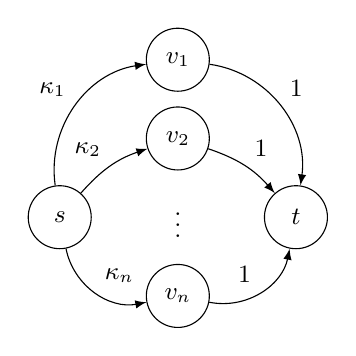
\begin{tikzpicture}[auto, node distance=1cm]
				      \tikzset{align=center,font=\small}
				      \tikzset{vertex/.style = {shape=circle,draw,minimum size=0.8cm}}
				      \tikzset{edge/.style = {-,> = latex'}}

				      \node[vertex] (1) {$s$};
				      \node[vertex] (2) [xshift=2cm,right of=1] {$t$};
				      \node (3) at ($(1)!0.5!(2)$) {\vdots};
				      \node[vertex] (5) [above of=3] {$v_2$};
				      \node[vertex] (4) [above of=5] {$v_1$};
				      \node[vertex] (6) [below of=3] {$v_n$};


				      \path[every node/.style={font=\sffamily\small}, every edge/.style={draw=black,->,> = latex}]
				      (1) edge[bend left=45] node {$\kappa_1$} (4)
				      (1) edge[bend left=15] node {$\kappa_2$} (5)
				      (1) edge[bend right=45] node {$\kappa_n$} (6)
				      (4) edge[bend left=45] node {$1$} (2)
				      (5) edge[bend left=15] node {$1$} (2)
				      (6) edge[bend right=45] node {$1$} (2)
				      ;

			      \end{tikzpicture}
		      \end{center}
		      The source node $s$ is connected directly to the sink node $t$ by multiple edges, each corresponding to a base kernel $\kappa_i$. The kernel for the entire graph $\mathcal{G}$ is the sum of all path kernels from $s$ to $t$, which corresponds to $\sum_{i=1}^n \kappa_i$ since each path kernel is essentially a base kernel.

		      \newpage
		      To construct a graph $\mathcal{G}$ such that the graph kernel $\kappa_{\mathcal{G}} = \prod_{i=1}^n \kappa_i$:

		      \textbf{Nodes}: We will create a sequence of nodes $u_0, u_1, \ldots, u_n$ where $u_0 = s$ and $u_n = t$.

		      \textbf{Edges}: We will add directed edges $u_{i-1} \to u_i$ with the base kernel $\kappa_i$.
		      \begin{center}
			      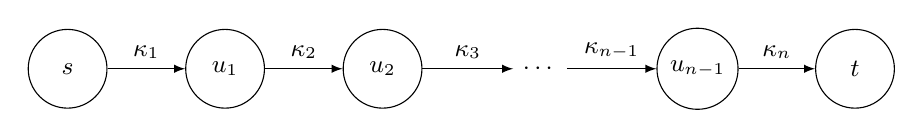
\begin{tikzpicture}[auto, node distance=2cm]
				      \tikzset{align=center,font=\small}
				      \tikzset{vertex/.style = {shape=circle,draw,minimum size=1cm}}
				      \tikzset{edge/.style = {-,> = latex'}}

				      \node[vertex] (1) {$s$};
				      \node[vertex] (2) [right of=1] {$u_1$};
				      \node[vertex] (3) [right of=2] {$u_2$};
				      \node[vertex] (5) [xshift=2cm,right of=3] {$u_{n-1}$};
				      \node (4) at ($(3)!0.5!(5)$) {$\cdots$};
				      \node[vertex] (6) [right of=5] {$t$};

				      \path[every edge/.style={draw=black,->,> = latex}]
				      (1) edge node {$\kappa_1$} (2)
				      (2) edge node {$\kappa_2$} (3)
				      (3) edge node {$\kappa_3$} (4)
				      (4) edge node {$\kappa_{n-1}$} (5)
				      (5) edge node {$\kappa_n$} (6);
			      \end{tikzpicture}
		      \end{center}

		      We have a linear sequence of nodes where each edge represents a base kernel $\kappa_i$. The kernel for the entire graph $\mathcal{G}$ is the only path kernel from $s$ to $t$, which corresponds to $\prod_{i=1}^n \kappa_i$.

		\item (1 pt) Consider the subgragh of the figure below that includes nodes $s, a, b, c$ (and arcs connecting them). \uline{Compute} the graph kernel where $s$ and $c$ play the role of source and sink, respectively. \uline{Repeat the computation} with the subgraph that includes $s, a, b, c, d$ (and arcs connecting them), where $d$ is the sink now.

		      \begin{center}
			      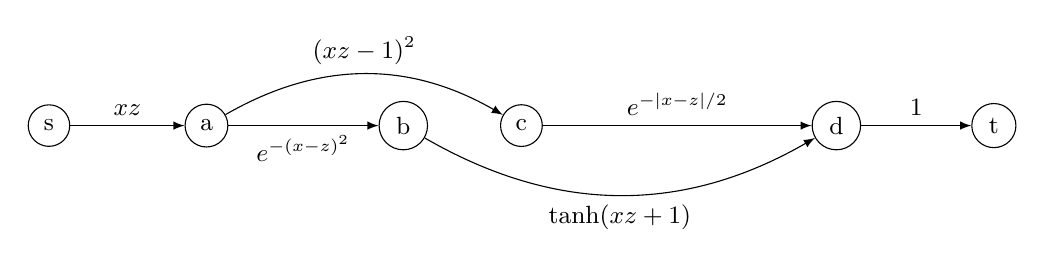
\begin{tikzpicture}[auto]
				      \tikzset{align=center,font=\small}

				      \tikzset{vertex/.style = {shape=circle,draw,minimum size=1.5em}}

				      \tikzset{edge/.style = {-,> = latex'}}

				      % vertices

				      \node[vertex] (s) at  (0,0) {s};

				      \node[vertex] (a) at  (2,0) {a};

				      \node[vertex] (b) at  (4.5,0) {b};

				      \node[vertex] (c) at  (6,0) {c};

				      \node[vertex] (d) at  (10,0) {d};

				      \node[vertex] (t) at  (12,0) {t};
				      %edges

				      \begin{scope}[every edge/.style={draw=black,->,> = latex}]
					      \draw[edge] (s) edge node{$xz$}  (a);
					      \draw[edge] (a) edge node[below] {$e^{-(x-z)^2}$}  (b);
					      \draw[edge] [bend left] (a) edge node {$(xz-1)^2$}  (c);
					      \draw[edge] [bend right] (b) edge node[below]{$\tanh(xz+1)$}  (d);
					      \draw[edge] (c) edge node{$e^{-|x-z|/2}$}  (d);
					      \draw[edge] (d) edge node{1}  (t);
				      \end{scope}
			      \end{tikzpicture}
		      \end{center}

		      \ans\\
		      \leavevmode\\
		      Subgraph 1: Nodes $s, a, b, c$, with $s$ as the source and $c$ as the sink

		      \textbf{Paths from $s$ to $c$}: $s \to a \to c$
		      $$
			      \kappa_{s \to a \to c}(x, z) = \kappa_{s \to a}(x, z) \cdot \kappa_{a \to c}(x, z) = xz(xz - 1)^2
		      $$
		      Thus,
		      $$
			      \boxed{\kappa_{\mathcal{G}_{s, c}}(x, z) = \kappa_{s \to a \to c}(x, z) = xz \cdot (xz - 1)^2}
		      $$

		      Subgraph 2: Nodes $s, a, b, c, d$, with $s$ as the source and $d$ as the sink

		      \textbf{Paths from $s$ to $d$}:
		      \begin{itemize}
			      \item Path 1: $s \to a \to b \to d$
			      \item Path 2: $s \to a \to c \to d$
		      \end{itemize}
		      Path 1: $s \to a \to b \to d$
		      $$
			      \kappa_{s \to a \to b \to d}(x, z) = \kappa_{s \to a}(x, z) \cdot \kappa_{a \to b}(x, z) \cdot \kappa_{b \to d}(x, z) = xz \cdot e^{-(x - z)^2} \cdot \tanh(xz + 1)
		      $$
		      Path 2: $s \to a \to c \to d$
		      $$
			      \kappa_{s \to a \to c \to d}(x, z) = \kappa_{s \to a}(x, z) \cdot \kappa_{a \to c}(x, z) \cdot \kappa_{c \to d}(x, z) = xz \cdot (xz - 1)^2 \cdot e^{-|x - z| / 2}
		      $$
		      Thus,
		      $$\boxed{
				      \begin{aligned}
					      \kappa_{\mathcal{G}_{s, d}}(x, z)
					      = & \kappa_{s \to a \to b \to d}(x, z) + \kappa_{s \to a \to c \to d}(x, z)                       \\
					      = & xz \cdot \left( e^{-(x - z)^2} \cdot \tanh(xz + 1) + (xz - 1)^2 \cdot e^{-|x - z| / 2}\right)
				      \end{aligned}
			      }
		      $$

		      \newpage
		\item (2 pts) \uline{Find an efficient algorithm to compute the graph kernel} $\kappa_{\mathcal{G}}(\xv, \zv)$ (for two fixed inputs $\xv$ and $\zv$) in time $O(|V| + |E|)$, assuming each base kernel $\kappa_e$ costs $O(1)$ to evaluate. You may assume there is always at least one $s-t$ path. State and justify your algorithm is enough; no need (although you are encouraged) to give a full pseudocode.

			      [Note that the total number of paths in a DAG can be exponential in terms of the number of nodes $|V|$, so naive enumeration would not work. For example, replicating the intermediate nodes in the above figure $n$ times creates $2^n$ paths from $s$ to $t$.]

			      [Hint: Recall that we can use \href{https://en.wikipedia.org/wiki/Topological_sorting}{topological sorting} to rearrange the nodes in a DAG such that all arcs go from a ``smaller'' node to a ``bigger'' one.]

		      \ans\\
		      \begin{algorithm}[H]
			      \DontPrintSemicolon
			      \KwIn{DAG $\mathcal{G} = (V, E)$, base kernels $\kappa_e$ for each edge $e \in E$, inputs $\xv, \zv$}
			      \KwOut{Graph kernel $\kappa_{\mathcal{G}}(\xv, \zv)$}

			      Perform a topological sort of the nodes in $V$ and store the sorted nodes in a list $L$\;

			      Initialize $\text{kernel}[v] \gets 0$ for all $v \in V$\;
			      $\text{kernel}[s] \gets 1$\tcp*{The kernel from the source to itself is 1}

			      \For{each node $u$ in $L$} {
				      \For{each neighbor $v$ of $u$} {
					      $\text{kernel}[v] \gets \text{kernel}[v] + \text{kernel}[u] \cdot \kappa_{u \to v}(\xv, \zv)$\;
				      }
			      }

			      \Return $\text{kernel}[t]$\tcp*{The graph kernel from $s$ to $t$}
			      \caption{Efficient Graph Kernel Computation in a DAG}
			      \label{alg:graph_kernel}
		      \end{algorithm}
		      \textbf{Topological Sorting}:
		      \begin{itemize}
			      \item Purpose: Ensures that each node $u$ is processed before any of its descendants $v$. This property is crucial for dynamic programming on a DAG as it guarantees that when we compute the value for a node, all values of its predecessors have already been computed.
			      \item Time Complexity: $O(|V| + |E|)$.
		      \end{itemize}

		      \textbf{Dynamic Programming}:
		      \begin{itemize}
			      \item Purpose: By summing the contributions of all incoming edges for each node, the algorithm correctly accumulates the kernel values for all paths from $s$ to $v$, ensuring that kernel[$t$] will contain the sum of the kernel values for all paths from $s$ to $t$.
			      \item Time Complexity: Each edge $(u \to v)$ is processed exactly once, and updating the kernel value for each edge takes $O(1)$ time. Therefore, the dynamic programming step also takes $O(|V| + |E|)$ time.
		      \end{itemize}

		      \textbf{Overall Time Complexity}: $O(|V| + |E|)$
	\end{enumerate}
\end{exercise}

\newpage
\begin{exercise}[CNN Implementation (8 pts)]
	\blue{\textbf{Note}: Please mention your Python version (and maybe the version of all other packages).}

	In this exercise you are going to run some experiments involving CNNs. You need to know \href{https://www.python.org/}{\magenta{Python}} and install the following libraries: \href{https://pytorch.org/get-started/locally/}{\magenta{Pytorch}}, \href{https://matplotlib.org/}{\magenta{matplotlib}} and all their dependencies. You can find detailed instructions and tutorials for each of these libraries on the respective websites.

	For all experiments, running on CPU is sufficient. You do not need to run the code on GPUs, although you could, using for instance \href{https://colab.research.google.com/}{Google Colab}.
	Before start, we suggest you review what we learned about each layer in CNN, and read at least this \href{https://pytorch.org/tutorials/beginner/blitz/neural_networks_tutorial.html}{\magenta{tutorial}}.

	\begin{enumerate}
		\item Implement and train a VGG11 net on the \href{https://pytorch.org/vision/stable/datasets.html#mnist}{\magenta{MNIST}} dataset.
		      VGG11 was an earlier version of VGG16 and can be found as model A in Table 1 of this \href{https://arxiv.org/pdf/1409.1556.pdf}{\magenta{paper}}, whose Section 2.1 also gives you all the details about each layer.
		      The goal is to get the loss as close to 0 as possible. Note that our input dimension is different from the VGG paper. You need to resize each image in MNIST from its original size $28 \times 28$ to $32 \times 32$ [why?].

		      For your convenience, we list the details of the VGG11 architecture here.
		      The convolutional layers are denoted as \texttt{Conv(number of input channels, number of output channels, kernel size, stride, padding)};
		      the batch normalization layers  are denoted as \texttt{BatchNorm(number of channels)};
		      the max-pooling layers are denoted as \texttt{MaxPool(kernel size, stride)};
		      the fully-connected layers are denoted as \texttt{FC(number of input features, number of output features)};
		      the drop out layers are denoted as \texttt{Dropout(dropout ratio)}:
		      \begin{verbatim}
			- Conv(001, 064, 3, 1, 1) - BatchNorm(064) - ReLU - MaxPool(2, 2)
			- Conv(064, 128, 3, 1, 1) - BatchNorm(128) - ReLU - MaxPool(2, 2)
			- Conv(128, 256, 3, 1, 1) - BatchNorm(256) - ReLU
			- Conv(256, 256, 3, 1, 1) - BatchNorm(256) - ReLU - MaxPool(2, 2)
			- Conv(256, 512, 3, 1, 1) - BatchNorm(512) - ReLU
			- Conv(512, 512, 3, 1, 1) - BatchNorm(512) - ReLU - MaxPool(2, 2)
			- Conv(512, 512, 3, 1, 1) - BatchNorm(512) - ReLU
			- Conv(512, 512, 3, 1, 1) - BatchNorm(512) - ReLU - MaxPool(2, 2)
			- FC(0512, 4096) - ReLU - Dropout(0.5)
			- FC(4096, 4096) - ReLU - Dropout(0.5)
			- FC(4096, 10)
			\end{verbatim}
		      You should use the \href{https://pytorch.org/docs/master/generated/torch.nn.CrossEntropyLoss.html}{cross-entropy loss} \verb|torch.nn.CrossEntropyLoss| at the end.

			      [This experiment will take up to 1 hour on a CPU, so please be cautious of your time. If this running time is not bearable, you may cut the training set to 1/10, so only have $\sim$600 images per class instead of the regular $\sim$6000.]

		      \ans\\
		      \leavevmode\\
		      Implemented in \texttt{cnn.py}.
		      \vspace{0.5cm}

		\item (4 pts) Once you've done the above, the next goal is to inspect the training process. \uline{Create the following plots}:
		      \begin{enumerate}
			      \item (1 pt) test accuracy vs the number of epochs (say 3 $\sim$ 5)
			      \item (1 pt) training accuracy vs the number of epochs
			      \item (1 pt) test loss vs the number of epochs
			      \item (1 pt) training loss vs the number of epochs
		      \end{enumerate}
		      [If running more than 1 epoch is computationally infeasible, simply run 1 epoch and try to record the accuracy/loss after every few minibatches.]

		      \ans{%
			      \begin{center}
				      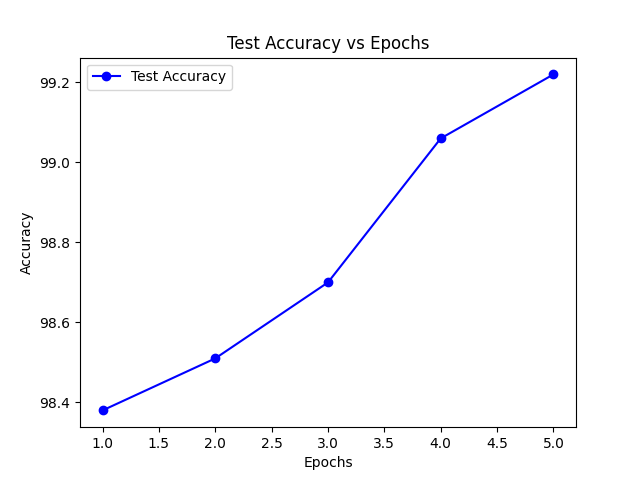
\includegraphics[width=.4\textwidth]{plots/test_accuracy_vs_epochs.png}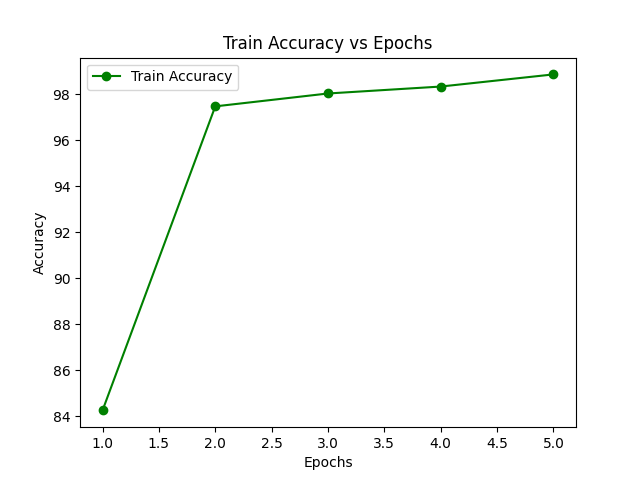
\includegraphics[width=.4\textwidth]{plots/train_accuracy_vs_epochs.png}\\
				      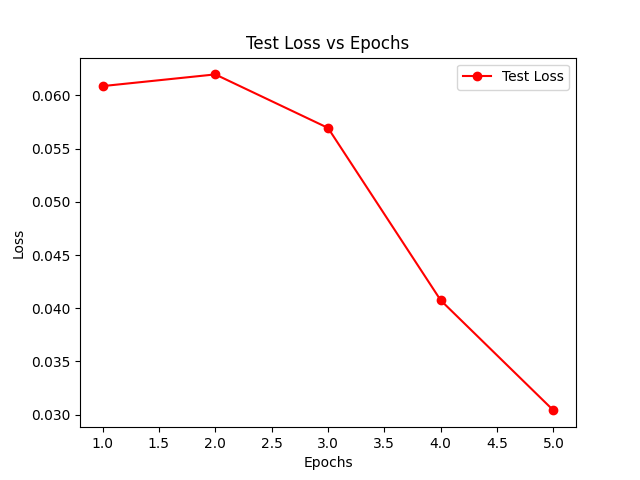
\includegraphics[width=.4\textwidth]{plots/test_loss_vs_epochs.png}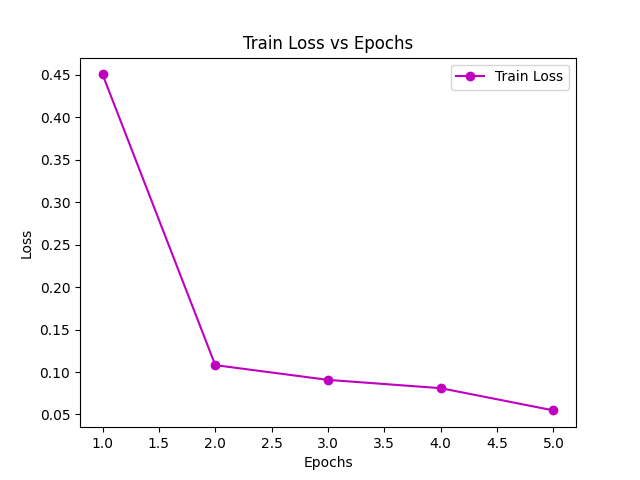
\includegraphics[width=.4\textwidth]{plots/train_loss_vs_epochs.png}\\
			      \end{center}
		      }

		\item Then, it is time to inspect the generalization properties of your final model. Flip and blur the \red{test set images} using any python library of your choice, and complete the following:
		      \begin{enumerate}[resume]
			      \item (1 pt) test accuracy vs type of flip. Try the following two types of flipping: flip each image from left to right, and from top to bottom. \uline{Report the test accuracy after each flip. What is the effect?}

			            You can read this \href{https://pytorch.org/vision/stable/transforms.html}{\magenta{doc}} to learn how to build a complex transformation pipeline. We suggest the following command for performing flipping:
			            \begin{verbatim}
				torchvision.transforms.RandomHorizontalFlip(p=1)
				torchvision.transforms.RandomVerticalFlip(p=1)
				\end{verbatim}

			            \ans{We can see that
				            \begin{center}
					            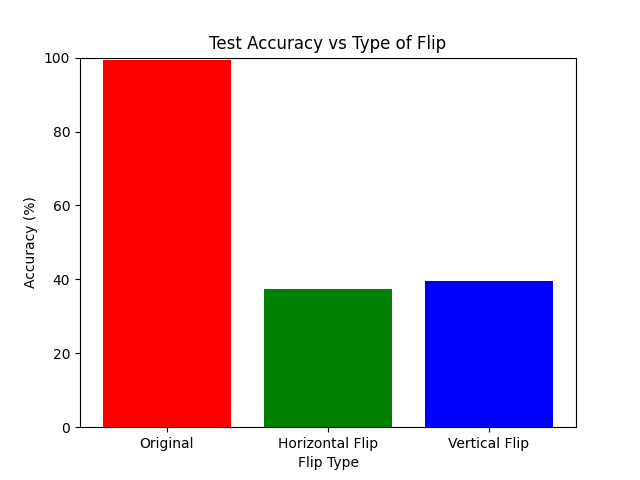
\includegraphics[width=.5\textwidth]{plots/accuracy_vs_flip.png}
				            \end{center}
			            }

			      \item (1 pt) test accuracy vs Gaussian noise. Try adding standard Gaussian noise to each test image with variance 0.01, 0.1, 1 and \uline{report the test accuracies. What is the effect?}

			            For instance, you may apply a user-defined lambda as a new transform t which adds Gaussian noise with variance say 0.01:
			            \begin{verbatim}
				t = torchvision.transforms.Lambda(lambda x : x + 0.1*torch.randn_like(x))
				\end{verbatim}

			            \ans{We can see that
				            \begin{center}
					            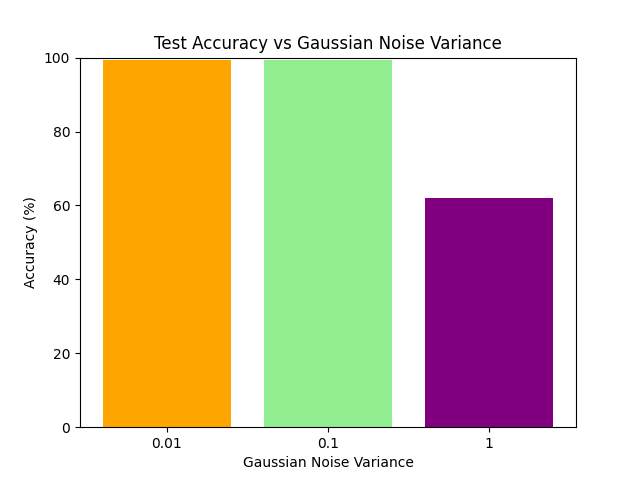
\includegraphics[width=.5\textwidth]{plots/accuracy_vs_noise.png}
				            \end{center}
			            }
		      \end{enumerate}

		\item (2 pts) Lastly, let us verify the effect of regularization. Retrain your model with data augmentation and test again as in item~3 above (both e and f). \uline{Report the test accuracy and explain} what kind of data augmentation you use in retraining.

		      \ans\\
		      \leavevmode\\
		      Training with the following data augmentations (randomly selected for each batch):
		      \begin{verbatim}
				transforms.RandomHorizontalFlip(p=1),
				transforms.RandomVerticalFlip(p=1),
				transforms.Lambda(lambda x: x + 1*torch.randn_like(x)),
				transforms.Lambda(lambda x: x + 0.1*torch.randn_like(x)),
				transforms.Lambda(lambda x: x + 0.01*torch.randn_like(x))
			\end{verbatim}
		      \begin{center}
			      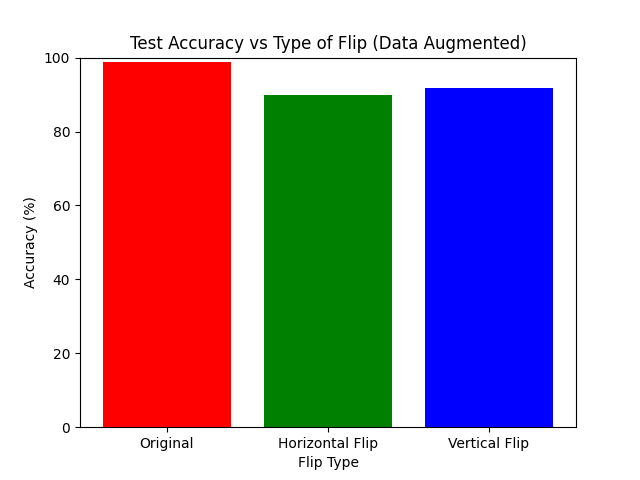
\includegraphics[width=.4\textwidth]{plots_retrained/accuracy_vs_flip.png}	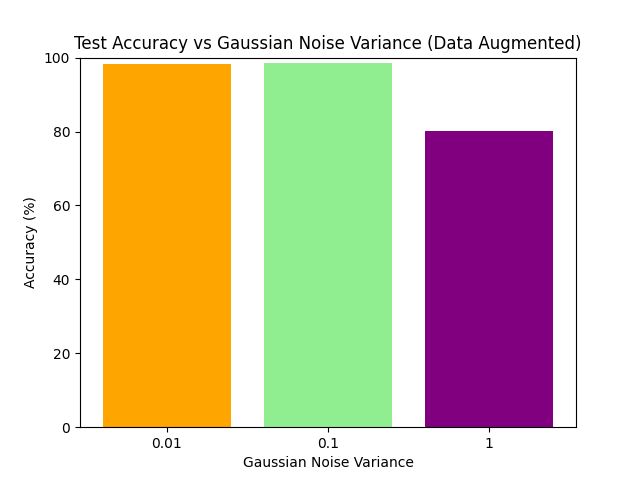
\includegraphics[width=.4\textwidth]{plots_retrained/accuracy_vs_noise.png}
		      \end{center}
	\end{enumerate}
\end{exercise}

\newpage
\begin{exercise}[Regularization (4 pts)]
	\blue{\textbf{Notation}: For the vector $\xv_i$, we use $x_{ji}$ to denote its $j$-th element.}

	Overfitting to the training set is a big concern in machine learning. One simple remedy is through injecting noise: we randomly perturb each training data before feeding it into our machine learning algorithm. In this exercise you are going to prove that injecting noise to training data is essentially the same as adding some particular form of regularization. We use least-squares regression as an example, but the same idea extends to other models in machine learning almost effortlessly.

	Recall that least-squares regression aims at solving:
	\begin{align}
		\label{eq:lr}
		\min_{\wv\in \RR^d} ~ \sum_{i=1}^n (y_i - \wv^\top\xv_i )^2,
	\end{align}
	where $\xv_i \in \RR^d$ and $y_i \in \RR$ are the training data. (For simplicity, we omit the bias term here.) Now, instead of using the given feature vector $\xv_i$, we perturb it first by some independent noise $\epsilonv_i$ to get $\tilde{\xv}_i = f(\xv_i, \epsilonv_i)$, with different choices of the perturbation function $f$. Then, we solve the following \textbf{expected} least-squares regression problem:
	\begin{align}
		\label{eq:plr}
		\min_{\wv\in \RR^d} ~ \sum_{i=1}^n \mathbf{E}[(y_i - \wv^\top\tilde\xv_i )^2],
	\end{align}
	where the expectation removes the randomness in $\tilde \xv_i$ (due to the noise $\epsilonv_i$), and we treat $\xv_i, y_i$ as fixed here. [To understand the expectation, think of $n$ as so large that we have each data appearing repeatedly many times in our training set.]

	\begin{enumerate}
		\item (2 pts) Let $\tilde{\xv}_i = f(\xv_i, \epsilonv_i) = \xv_i + \epsilonv_i$ where $\epsilonv_i \sim \mathcal{N}(\zero, \lambda I)$ follows the standard Gaussian distribution. Simplify \eqref{eq:plr} as the usual least-squares regression \eqref{eq:lr}, plus a familiar regularization function on $\wv$.

		      \ans\\
		      \leavevmode\\
		      Substituting $\tilde{\xv}_i = \xv_i + \epsilonv_i$, we have:
		      $$
			      \begin{aligned}
				      (y_i - \wv^\top \tilde{\xv}_i)^2
				      = & (y_i - \wv^\top (\xv_i + \epsilonv_i))^2                                                            \\
				      = & (y_i - \wv^\top \xv_i - \wv^\top \epsilonv_i)^2                                                     \\
				      = & (y_i - \wv^\top \xv_i)^2 - 2(y_i - \wv^\top \xv_i)(\wv^\top \epsilonv_i) + (\wv^\top \epsilonv_i)^2
			      \end{aligned}.
		      $$

		      Thus,

		      $$
			      \mathbf{E}[(y_i - \wv^\top \tilde{\xv}_i)^2] = \mathbf{E}[(y_i - \wv^\top \xv_i)^2] - 2\mathbf{E}[(y_i - \wv^\top \xv_i)(\wv^\top \epsilonv_i)]+\mathbf{E}[(\wv^\top \epsilonv_i)^2].
		      $$

		      Taking the expectation of each term separately:

		      1. $\mathbf{E}[(y_i - \wv^\top \xv_i)^2] = (y_i - \wv^\top \xv_i)^2$, since this term is deterministic with respect to the noise.

		      2. $\mathbf{E}[(y_i - \wv^\top \xv_i)(\wv^\top \epsilonv_i)] = (y_i - \wv^\top \xv_i) \mathbf{E}[\wv^\top \epsilonv_i] = 0$, because $\epsilonv_i$ has zero mean.

		      3. $\mathbf{E}[(\wv^\top \epsilonv_i)^2] = \wv^\top \mathbf{E}[\epsilonv_i \epsilonv_i^\top] \wv = \wv^\top (\lambda I) \wv = \lambda \|\wv\|^2_\mathrm{F}$.

		      Combining these results, we get:

		      $$
			      \mathbf{E}[(y_i - \wv^\top \tilde{\xv}_i)^2] = (y_i - \wv^\top \xv_i)^2 + \lambda \|\wv\|^2_\mathrm{F}.
		      $$

		      Therefore, the expected least-squares regression objective becomes:

		      $$
			      \boxed{\min_{\wv \in \RR^d} \sum_{i=1}^n \left( (y_i - \wv^\top \xv_i)^2 + \lambda \|\wv\|^2_\mathrm{F} \right)}.
		      $$

		      \newpage
		\item (2 pts) Let $\tilde{\xv}_i = f(\xv_i, \epsilonv_i) = \xv_i \odot \epsilonv_i$, where $\odot$ denotes the element-wise product and $p \epsilon_{ji} \sim \href{https://en.wikipedia.org/wiki/Bernoulli_distribution}{\magenta{\mathrm{Bernoulli}}}(p)$ \href{https://en.wikipedia.org/wiki/Independence_(probability_theory)}{\magenta{independently}} for each $j$. That is, with probability $1-p$ we reset $x_{ji} $ to 0 and with probability $p$ we scale $x_{ji}$ as $x_{ji}/p$. Note that for different training data $\xv_i$, $\epsilonv_i$'s are independent. Simplify \eqref{eq:plr} as the usual least-squares regression \eqref{eq:lr}, plus a different regularization function on $\wv$ (that may also depend on $\xv$). [This way of injecting noise, when applied to the weight vector $\wv$ in a neural network, is known as Dropout (DropConnect).]

		      \ans\\
		      $$
			      \epsilon_{ji} =
			      \begin{cases}
				      \frac{1}{p} & \text{with probability } p,   \\
				      0           & \text{with probability } 1-p.
			      \end{cases}
		      $$
		      Then, each element of $\tilde{\xv}_i$ can be represented as:

		      $$
			      \tilde{x}_{ji} =
			      \begin{cases}
				      x_{ji} / p & \text{with probability } p,   \\
				      0          & \text{with probability } 1-p.
			      \end{cases}
		      $$

		      Substituting $\tilde{\xv}_i = \xv_i \odot \epsilonv_i$, we have:

		      $$
			      \begin{aligned}
				      (y_i - \wv^\top \tilde{\xv}_i)^2
				      = & \left(y_i - \sum_{j=1}^d w_j \tilde{x}_{ji}\right)^2                                                       \\
				      = & \left(y_i - \sum_{j=1}^d w_j x_{ji} \epsilon_{ji}\right)^2                                                 \\
				      = & y_i^2 - 2 y_i \sum_{j=1}^d w_j x_{ji} \epsilon_{ji} + \left(\sum_{j=1}^d w_j x_{ji} \epsilon_{ji}\right)^2
			      \end{aligned}.
		      $$

		      Thus,

		      $$
			      \mathbf{E}[(y_i - \wv^\top \tilde{\xv}_i)^2] = \mathbf{E}\left[y_i^2\right] - 2\mathbf{E}\left[y_i \sum_{j=1}^d w_j x_{ji} \epsilon_{ji}\right] + \mathbf{E}\left[\left(\sum_{j=1}^d w_j x_{ji} \epsilon_{ji}\right)^2\right].
		      $$

		      Taking the expectation of each term separately:

		      1. $\mathbf{E}[y_i^2] = y_i^2$.

		      2. $\mathbf{E}\left[y_i \sum_{j=1}^d w_j x_{ji} \epsilon_{ji}\right] = y_i \sum_{j=1}^d w_j x_{ji} \mathbf{E}[\epsilon_{ji}] = y_i \sum_{j=1}^d w_j x_{ji}=y_i\wv^\top \xv_i.$

		      3. With $\mathbf{E}[\epsilon_{ji}^2]=\frac{1}{p}$ and $\mathbf{E}[\epsilon_{ji}\epsilon_{ki}]=\mathbf{E}[\epsilon_{ji}]\mathbf{E}[\epsilon_{ki}]=1$,

		      $$
			      \begin{aligned}
				      \mathbf{E}\left[\left(\sum_{j=1}^d w_j x_{ji} \epsilon_{ji}\right)^2\right]
				      = & \sum_{j=1}^d w_j^2 x_{ji}^2 \mathbf{E}[\epsilon_{ji}^2] + \sum_{j\neq k}w_jw_kx_{ji}x_{ki}\mathbf{E}[\epsilon_{ji}\epsilon_{ki}] \\
				      = & \frac{1}{p}\sum_{j=1}^d w_j^2 x_{ji}^2 + \sum_{j\neq k}w_jw_kx_{ji}x_{ki}                                                        \\
				      = & \sum_{j=1}^d w_j^2 x_{ji}^2 + \sum_{j\neq k}w_jw_kx_{ji}x_{ki} + \frac{1-p}{p}\sum_{j=1}^d w_j^2 x_{ji}^2                        \\
				      = & (\wv^\top \xv_i)^2 + \frac{1-p}{p}\sum_{j=1}^d w_j^2 x_{ji}^2.
			      \end{aligned}
		      $$
		      \newpage
		      Combining these results, we get:

		      $$
			      \begin{aligned}
				      \mathbf{E}[(y_i - \wv^\top \tilde{\xv}_i)^2]
				      = & y_i^2 - 2 y_i \wv^\top \xv_i + (\wv^\top \xv_i)^2 + \frac{1-p}{p}\sum_{j=1}^d w_j^2 x_{ji}^2 \\
				      = & (y_i-\wv^\top \xv_i)^2 + \frac{1-p}{p}\sum_{j=1}^d w_j^2 x_{ji}^2.
			      \end{aligned}
		      $$

		      Therefore, the expected least-squares regression objective becomes:

		      $$
			      \boxed{\min_{\wv \in \RR^d} \sum_{i=1}^n\left(  (y_i-\wv^\top \xv_i)^2 + \frac{1-p}{p}\sum_{j=1}^d w_j^2 x_{ji}^2 \right)}.
		      $$
	\end{enumerate}
\end{exercise}
\end{document}
